\chapter{Methods}
\label{ch:methods}

\section{Overview}
\label{sec:overview}
In this section, we present an overview of the key components that make up our system as well as the different operational modes for evaluating the complete system's capabilities. Below summarizes the contents of this section, including the key components of our system and the different operational modes for evaluating its capabilities.
\begin{itemize}
  \item \textbf{LiDAR-based SLAM system:} The LiDAR-based SLAM system is our base system which comprises VILENS LiDAR-inertial odometry~\cite{wisth2023tro} for state estimation and the pose graph SLAM~\cite{proudman2022ras} for achieving accurate localization and mapping. However, this system accumulates drift over time.
  \item \textbf{Place recognition server:} The place recognition server enables robust detection and verification of loop closures. This allows the SLAM system to correct the accumulated drift, improving the overall accuracy of the map (main focus of this project).
 
  \item \textbf{Evaluation of three different operational modes:} We introduce three different operational modes: online SLAM, offline multi-mission SLAM map merging, and relocalization modes. This will demonstrate capabilities of our system in various scenarios and highlight the importance of place recognition for achieving consistent and accurate maps. 
\end{itemize}

\section{LiDAR SLAM system}
The LiDAR-based SLAM system is the base system that provides the robot's pose estimate and the 3D map of the environment. The system consists of two main components: state estimation module (LiDAR-inertial odometry) and pose graph SLAM system. The state estimation module provides the robot's incremental pose estimate based on the local sensor measurements around the mapping device. The pose graph SLAM system is used to optimize the robot's pose estimate globally correcting the accumulated drift from the state estimation module. We will provide a overview of the odometry system and the pose graph SLAM system in the following paragraphs. 
\vspace{6pt}

\noindent \textbf{LiDAR-intertial odometry} \hspace{0.5em} For the state estimation, we use a LiDAR-intertial factor graph-based odometry system, VILENS~\cite{wisth2023tro} to provide a continuous odometry estimate at high frequency. VILENS uses four sensor modalities IMU, LiDAR, camera, and (leg kinematics) being tightly coupled in a factor graph as shown in \figref{fig:vilens_factorgraph} (Left). But in this project, we only used IMU and LiDAR sensors, which are sufficient for tracking the pose when running inside forest environments. 
The state estimation problem can be formulated as maximum a posteriori (MAP) problem for estimating all states $\mathbf{X}_k$, by optimizing over all states $\mathbf{X}_k$ given all measurements $\mathbf{Z}_k$ up to time $k$ as follows: 
\begin{equation}
  \begin{aligned}
  &\mathbf{X}_k = \arg\max_{\mathbf{X}_k} p(\mathbf{X}_k|\mathbf{Z}_k) \propto p(\mathbf{X}_0) p(\mathbf{Z}_k|\mathbf{X}_k) \\
  &\quad= \arg\min_{\mathbf{X}_k} -\log p(\mathbf{X}_0) -\log p(\mathbf{Z}_k|\mathbf{X}_k)
  \end{aligned}
\end{equation}
Assuming each measurement is conditionally independent with the effect of Gaussian noise, the optimization problem can be formulated as least squares problem:   
\begin{equation}
  \mathbf{X}_k = \arg\min_{\mathbf{X}_k} \| \mathbf{r}_0 \|^2 + \sum_{i \in K_k} \left( \| \mathbf{r}^{\text{I}}_{ij} \|_{\Sigma_{\mathbf{r}^{\text{I}}_{ij}}}^2 + \| \mathbf{r}^{\text{L}}_{i} \|_{\Sigma_{\mathbf{r}^{\text{L}}_{i}}}^2  \right)
\end{equation}\label{eq:least_square}
where $\mathbf{r}_0$, $\mathbf{r}^{\text{I}}_{ij}$, and $\mathbf{r}^{\text{L}}_{i}$ are residual error associated with prior, IMU preintegration factor, and LiDAR factor at key frame $i$ respectively. IMU measurements are preintegrated to the pose and velocity between two consecutive nodes of the graph to provide position, velocity, and orientation. The LiDAR registration factor is used to compute the relative difference transformation between two LiDAR scans from estimated poses and ICP using Iterative Closest Point (ICP). This optimization problem is solved using the iSAM2 algorithm~\cite{Kaess2012}, which will be explained in the next section. 

This LiDAR-inertial odometry system is used to provide a locally consistent estimate of the robot's pose. However, the system can suffer from accumulated drift over time. An example of the drift accumulation is shown in \figref{fig:odometry_slam}. After a long traverse in the forest and return to the starting point, we can see that the odometry path diverges from the starting point (yellow line). The pose graph SLAM system (green line) is used to correct this drift by finding a suitable loop closure constraint (red line). \vspace{6pt}


\begin{figure}[t]
  \centering
  \includegraphics[width=\columnwidth]{pics/methods_vilens_factorgraph2.pdf}
  \caption{Left: VILENS odometry system as a factor graph representation. The factors are: prior (black), visual
 (yellow), lidar planes (green), lidar lines (red), preintegrated IMU (orange), preintegrated velocity (from leg kinematics, blue), and lidar odometry from ICP registration (magenta). State nodes are white, while landmarks are grey. In forest environments, only LiDAR odometry and IMU factors are used without visual factors. Right: Pose graph SLAM. The system optimizes the poses after successful loop closure verification. The pose graph is constructed from odometry factors and loop closure factors.}
  \label{fig:vilens_factorgraph}
\end{figure}

\begin{figure}[htbp]
  \centering
  \includegraphics[width=0.8\columnwidth]{pics/methods_odometry_slam.pdf}
  \caption{Illustrative visualization of both odometry and SLAM paths after a long traverse in Wytham Woods. The odometry path is shown in yellow line and the optimized SLAM path is shown in green. The SLAM path successfully minimized the odometry drift after a loop closure (red line) is found when the mapping device returned to the starting point.}
  \label{fig:odometry_slam}
\end{figure}

\noindent \textbf{Pose graph SLAM}\hspace{0.5em}  We use a pose graph SLAM system to optimize the robot's pose estimate. The pose graph is constructed from odometry factors and loop closure factors as shown in \figref{fig:vilens_factorgraph} (Right). Each node contains a LiDAR scan and corresponding pose, and the edge is formed between consecutive nodes from incremental odometry estimates. Each loop closure adds another constraint between two nodes. The odometry factors are provided by VILENS, while the loop closure factors are obtained using the place recognition server developed during this project. The pose graph is optimized using the iSAM2~\cite{Kaess2012} algorithm as well. \\

\noindent \textbf{Pose graph optimization}\hspace{0.5em} iSAM~\cite{Kaess2012}(Incremental Smoothing and Mapping) is used to solve the least square minimization problem in pose graph SLAM when a new loop constraint is added. The pose graph optimization is formulated as non-linear least square problem:
\begin{equation}
  F(\mathbf{x}) = \min_{\mathbf{x}} \sum_{(i,j) \in E} \| \mathbf{r}_{ij} \|_{\Sigma_{\mathbf{r}_{ij}}}^2 + \sum_{(k,l) \in L} \| \mathbf{r}_{kl} \|_{\Sigma_{\mathbf{r}_{kl}}}^2
\end{equation}  
where $\textbf{x}$ represent all poses and $\mathbf{r}_{ij}$ is the odometry residual error and $\mathbf{r}_{kl}$ is the loop closure residual error. Since this is non-linear least square problem, it should be solved by linearising the residual error using the first order Taylor approximation around the current guess $\mathbf{x}_0$ as follows: 
\begin{equation}
  \mathbf{r}_{ij}(\mathbf{x}_0 + \Delta \mathbf{x}) \approx \mathbf{r}_{ij}(\mathbf{x}_0) + \mathbf{J}_{ij} \Delta \mathbf{x} 
\end{equation}
Substituting back to the original $F(\mathbf{x})$, 
\begin{equation}
  \begin{aligned}
      F(\mathbf{x}_0 + \Delta \mathbf{x}) &= \sum\limits_{i,j \in E,L} \biggl( \mathbf{r}_{ij}(\mathbf{x}_0)^T \Sigma_{\mathbf{r}_{ij}} \mathbf{r}_{ij}(\mathbf{x}_0) \\
      &\quad + 2 (\Delta \mathbf{x})^T \mathbf{J}_{ij}^T \Sigma_{\mathbf{r}_{ij}} \mathbf{r}_{ij}(\mathbf{x}_0) + (\Delta \mathbf{x})^T \mathbf{J}_{ij}^T \Sigma_{\mathbf{r}_{ij}} \mathbf{J}_{ij} \Delta \mathbf{x} \biggr)
  \end{aligned}
  \end{equation}
  \begin{equation}
  \begin{aligned}
      &= c + 2\mathbf{b}^T\Delta \mathbf{x} + \Delta \mathbf{x}^T H \Delta \mathbf{x}.
  \end{aligned}
\end{equation}
Then setting $\frac{\partial F}{\partial \Delta \mathbf{x}}=0$ gives:
\begin{equation}
  \begin{aligned}
  &\quad H \Delta \mathbf{x} = -\mathbf{b} 
  \end{aligned}
\end{equation}
Then iteratively solve $\mathbf{x*}=\mathbf{x_0} + \Delta \mathbf{x}$. Note that directly inverting the sparse information matrix $H$ is computationally expensive due to its size and infeasible to re-calculate every time when a new constraint is added. Instead, iSAM performs QR decomposition on the $H$ matrix, resulting in a sparse upper triangular matrix. This allows efficient incremental addition of a new constraint and reordering so that this update is computational efficient and real-time capable.  

In summary, the pose graph SLAM system is an essential component to maintain globally consistent poses and a map. When a loop closure is found, the pose graph SLAM optimizes the trajectory to minimize the effect of drift. As illustrated in \figref{fig:odometry_slam}, the odometry path (yellow line) tends to accumulate drift over time, while the optimized SLAM path (green line), after incorporating a loop closure constraint (red line), is able to correct this drift.
However, integrating an incorrect loop closure into the pose graph can lead to a failure in the entire SLAM system. Therefore, it is crucial to have a reliable place recognition system as a front-end component, responsible for providing verified loop closure candidates. In the following section, we will discuss \emph{ place recognition server} which is responsible for providing reliable loop closure candidates to the pose graph SLAM system.


% Overall Pipeline
% This star removes this subsection from the A,B,C list. Such that the task A,B,C match
\section{Place Recognition \& Verification Server} \label{sec:pipeline}
The focus of the research in this report is on the place recognition
server. Our place recognition pipeline (\figref{fig:pipeline}) consists of three steps: loop candidate proposals, coarse registration, and a final fine-registration. At each step, we perform appropriate checks to filter out incorrect loop closures.

The main inputs are the pose graph, with corresponding LiDAR scans attached to each pose, as well as the single query scan. The query scan is provided by different sources depending on the task we are solving. For example, in the relocalization task it will be a live scan directly from the LiDAR sensor. Further details are provided in the corresponding sections.
\begin{figure}[t]
  \centering
  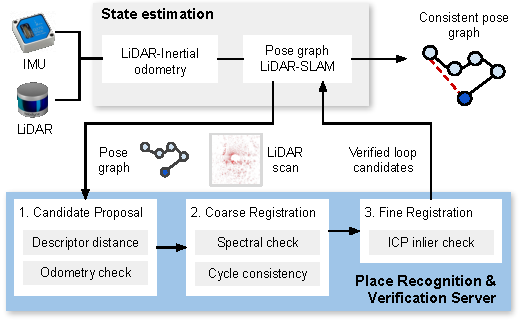
\includegraphics[width=\columnwidth]{pics/method_pipeline.pdf}
  \caption{Our place recognition pipeline. Grey components: base state estimation modules. Blue components: place recognition server (the focus of the research in this project). VILENS provides a continuous odometry estimate at 10 Hz. Pose graph SLAM is used to optimize poses after successful loop closure verification. 
  The place recognition module consists of three steps: Loop candidate proposal, coarse registration, and fine registration. We verify loop candidates
  at the global descriptor-level, local feature-level consistency, and finally fine registration level. A loop candidate is integrated in the pose graph only if it passes these three stages.}
  \label{fig:pipeline}
\end{figure}

% 1.1 Descriptors (Descriptor distance,)
\subsection*{\textbf{Step 1: Loop candidate proposals}}
\label{subsubsec:loop-candidate}
\begin{figure}[htbp]
  \centering
  \includegraphics[width=\columnwidth]{pics/methods_fig_descriptor3.pdf}
  \caption{Different types of place recognition descriptors on Wild-Place~\cite{knights2023icra} data. Left: ScanContext, Middle: STD, Right: EgoNN and Logg3dNet(Right). ScanContext encodes maximum height at each sector defined by radius and angle. This information is then transformed into a 2D descriptor where the horizontal axis represents the angle and the vertical axis represents the radius. STD computes corners of planes (in our case the trunks of trees) and connects them to form triangle cliques which can be quickly matched. EgoNN and Logg3dNet both compute learning-based pointwise descriptors in voxelized point clouds coloured by similar point features.}
  \label{fig:descriptors_example}
\end{figure}
Initial loop closure candidates are obtained by comparing global descriptors extracted from the pose graph scans as well as the query scan. In this thesis, we evaluate four state-of-the-art methods for descriptor extraction: the learning-based Logg3dNet~\cite{vidanapathirana2022icra} and EgoNN~\cite{komorowski2022ral}, as well as the handcrafted ScanContext~\cite{kim2018iros} and STD~\cite{yuan2023icra}. \figref{fig:descriptors_example} shows their descriptors examples computed on Wild-Place data.  

Given the reference pose graph and the query scan, we compute a database of descriptors using all the scans in the pose graph, given by the matrix $\mathbf{D} \in \R{N\times M}$, where $N$ is the number of poses in the pose graph and $M$ the descriptor dimension. Additionally, we compute the descriptor for the query scan, denoted by $\mathbf{d}_{q} \in \R{M \times 1}$. 
To obtain candidates, we compute the pairwise descriptor distances of the scan to the database using the cosine similarity:
\begin{equation}
  \mathbf{S} = \mathbf{D} \cdot \mathbf{d}_{q} \in \R{N \times 1}
\end{equation}
The vector of descriptor distances $\mathbf{S}$ is sorted by increasing distance, and only the top-$k$ candidates are selecting using a distance threshold $\tau_{s}$, which is set by the $F_1$-max score from testing data.
If a spatial prior is available, for example from LiDAR-inertial odometry, we also perform an additional spatial check discarding all the candidates that are more than a (conservative) threshold distance of \SI{20}{\meter} away from the query scan. The output is a set of candidate nodes $\{ n_c\}$.


% 2.1 Pose Estimation (RANSAC) ... notation is a bit confusing.
\subsection*{\textbf{Step 2: Coarse Registration}}
\label{subsubsec:coarse-registration}
\begin{figure}[htbp]
  \centering
  \includegraphics*[width=\columnwidth]{pics/methods_registration_2.pdf}
  \caption{Registration example of two point clouds \SI{7.3}{\meter} and \SI{111}{\degree} apart. Left image is before registration. Right image shows after RANSAC-registration. After RANSAC-registration, the trunks of trees scans (Blue boxes) are clearly matched with each other . }
  \label{fig:registration_example}
\end{figure}
\noindent Next, we estimate the relative 6DoF transformation that expresses the pose associated to the query scan w.r.t each candidate node, which we denote $\Delta \mathbf{T}$. For the handcrafted methods (ScanContext and STD), the relative transformation is directly an output of descriptor computation. For the learning-based approaches, we use the point-wise feature vectors output in the forward pass of Logg3dNet and EgoNN for feature matching, which is used in a RANSAC-based pose estimation scheme~\cite{fischler1981ransac} to estimate the relative transformation. We used \emph{Open3D}'s RANSAC implementation~\cite{zhou2018}.  
% \vspace{6pt}
\begin{figure}[htbp]
  \centering
  \includegraphics*[width=0.9\columnwidth]{pics/methods_keypoint_matching.pdf}
  \caption{RANSAC matches obtained from Logg3dNet features for two examples: one with a small baseline distance and another with a large baseline distance. Left image shows short baseline distance \SI{0.8}{\meter} and \SI{6}{\degree} viewpoint difference and right image shows large baseline distance \SI{7}{\meter} and \SI{1}{\degree} viewpoint difference. 
  The red points represent keypoints in the query point cloud, while green points depict candidate keypoints in the retrieved point cloud. Each keypoint possesses its unique feature vector, matched against the most similar feature in the retrieved point clouds (indicated by black lines). In the left image, with a short baseline distance and minimal viewpoint difference, RANSAC matching consistently discovers matching pairs along the horizontal axis. However, in the right image, where the baseline distance is significantly larger, some outliers are depicted as a cluster of vertical lines in the figure.}
  \label{fig:RANSAC_keypoint_matching}
\end{figure}

\noindent \textbf{RANSAC Registration}\hspace{0.5em} \figref{fig:RANSAC_keypoint_matching} shows illustrative examples of RANSAC feature matchings. We noticed that as the distance between two point clouds increases, there are more incorrect matches (outliers) due to small amount of point-size overlap between them. This also suggests that RANSAC only measures if two point clouds can be registered but is unable to determine if a loop candidate is actually a false positive or a correct loop candidate but with far baseline distance. Because of this we then introduced two more verification layers, Spectral Geometric Verification (SGV) and pairwise cycle consistency check. 

\noindent \textbf{Spectral Geometric Verification (SGV)}\hspace{0.5em} We additionally verify the inlier matches using the \emph{Spectral Geometric Verification}(SGV)~\cite{vidanapathirana2023ral} method, which provides an additional measure of the quality of the feature matches. Essentially, SGV checks pairwise cycle consistency of local feature correspondences between two point clouds. Given the correspondences between two point clouds, $\mathcal{C}=\{c_1, c_2 \ldots c_n\}$ we can construct a graph $\mathbf{M} \in \R{n \times n}$ where $M_{i,j}$ represents similarity score $s$ between $c_i$ and $c_j$. If both $c_i$ and $c_j$ are correct inliers they should be pairwise consistent in their coordinate frames with high similarity score $s$, but if one of correspondences is an outlier they will not be consistent with low similarity score $s$. 
\begin{figure}[t]
  \centering
  \includegraphics*[width=0.8\columnwidth]{pics/methods_svg_distance2.png}
  \caption{The SGV scores $s$ are computed against baseline distances and angles of loop closures obtained (White bins are empty data points). A smaller SGV score corresponds to larger baseline distances, suggesting a reduced proportion of correct correspondences. 
  For example, $s=0.1$ approximately indicates \SI{10}{\meter} baseline distance, and $s=0.05$ indicates \SI{20}{\meter}. Furthermore, it was observed that the SGV score remains constant across different angles, indicating a consistent registration process irrespective of viewpoint changes (viewpoint invariant), and useful indication of baseline distance.}
  \label{fig:sgv_distance}
\end{figure}
For example, let's consider two correspondences $c_1 =\{\mathbf{p}_i^{A}, \mathbf{p}_l^{B}\}$, $c_2=\{\mathbf{p}_j^{A}, \mathbf{p}_k^{B}\}$ where $ \mathbf{p}\in \R{3}$ between two point clouds $A$ and $B$. The euclidean distance $\| \mathbf{p}_i^{A}-\mathbf{p}_j^{A} \|$ and $\| \mathbf{p}_k^{B}-\mathbf{p}_l^{B} \|$ should be consistent each other if they are both correct correspondences. Thus, the quality of the feature correspondences can be found by minimizing the error $d$ between these two distances: 
\begin{equation}
  d_{1,2} = \|\| \mathbf{p}_i^{A}-\mathbf{p}_j^{A} \| - \| \mathbf{p}_k^{B}-\mathbf{p}_l^{B} \| \| 
\end{equation}
\begin{equation}
  M_{1,2} = max( 0 , 1 - \left(\frac{d_{i,j}}{d_{\text{thres}}}\right)^2 ) 
  \quad \text{where} \quad 0 \leq M_{1,2} \leq 1 
\end{equation}
$d_{thres}$ typically set to \SI{0.1}{\meter} to \SI{0.2}{\meter} to consider the error in the registration process. If $d_{i,j}$ is larger than $d_{thres}$, we consider two correspondences are inconsistent and $M_{i,j}$ assigned to be zero.  
We then compute the total SGV score $s$ considering all correspondences $\mathcal{C}=\{c_1, c_2 \ldots c_n\}$ as follows:
\begin{equation}
  s = \sum_{i,j} M_{i,j} 
\end{equation}
By finding maximum inliers $\mathbf{v^{*}}$, we can find the maximum SGV score $s^{*}$: 
\begin{equation}
  \mathbf{v^{*}} = \argmax_{\mathbf{v}} \mathbf{v}^T \mathbf{M} \mathbf{v} \quad, \quad
  s^{*} = \mathbf{v}^{*T} \mathbf{M} \mathbf{v}^{*}
\end{equation}
where $\mathbf{v}$ is the eigenvector of the largest eigenvalue of $\mathbf{M}$. The SGV score $s$ is then used to verify the quality of the feature matches.

The authors of Logg3dNet proposed using the SGV check to re-ranking top-$k$ candidates obtained from descriptor distance matching in \secref{subsubsec:loop-candidate}. Instead we used SGV to verify registration quality against baseline distance. \figref{fig:sgv_distance} shows the SGV score computed against the distance between two point clouds. We used SGV score as an indication of baseline distance of loop candidates. For example, we set $s=0.1$ as a threshold for \SI{10}{\meter} baseline distance, and reject the loop candidates if SGV score is smaller than 0.1.


\begin{figure}[htbp]
  \centering
  \includegraphics*[width=0.7\columnwidth]{pics/methods_pairwise_consistency.pdf}
  \caption{Our proposed pairwise cycle consistency check is general and applies to the online and offline multi-mission SLAM case, as well as relocalization tasks. We only need the relative transformation estimates (from the odometry system) and loop candidates (from the place recognition server) between four nodes $n_i, n_j, n_k, n_l$ to verify the validity of a loop in the pose graph. Please refer to \secref{subsubsec:coarse-registration} for technical details.}
  \label{fig:cycle-consistency}
\end{figure}
\subsubsection*{\textbf{Pairwise Loop Closures Cycle Consistency Check}}
Lastly, we carry out a \emph{loop closure cycle consistency} verification (\figref{fig:cycle-consistency}), which checks whether the relative transformations between pairs of nodes in pose graph are mutually consistent with one another. Given four pose graph nodes $n_i, n_j, n_k, n_l$, we test how close the following equivalence holds:
\begin{equation}
\Delta\mathbf{T}_{i,j}\, \Delta\mathbf{T}_{j,k}\, \Delta\mathbf{T}_{k,l}\, \Delta\mathbf{T}_{l,i}\, \approx \mathbf{I}_{4\times4} 
\end{equation}
If this difference is more than a threshold of \SI{10}{\centi\meter} or \SI{1}{\degree} we reject the candidate. 

This is shown in \figref{fig:cycle-consistency}, the interpretation of these transformations change depending on operation modes: online SLAM (\secref{sec:online_slam_mode}), offline multi-mission SLAM (\secref{sec:offline}), or pure relocalization (\secref{sec:relocalization}). However, the main idea remains the same: to verify if two successive loop candidates are consistent across different frames (Alg.\ref{alg:pairwise_cycle_check} shows some pseudocodes for computing pairwise cycle consistency check).


\begin{algorithm}[htbp]
  \small
  \DontPrintSemicolon
  \SetAlgoLined
  \SetNoFillComment
  \LinesNotNumbered 
  \SetKwInOut{Input}{Input}
  \SetKwInOut{Output}{Output}
  
  \Input{$\Delta\mathbf{T}_{t}$ current loop closure}
  \Output{$success$ or $fail$ of the cycle consistency check}

  % % Comments describing the algorithm steps
  % \tcp{$n_i, n_j, n_k, n_l$: Nodes} 
  % \tcp{$\Delta\mathbf{T}_{t-1}$: Previous loop closure}
  % \tcp{$fails$: Number of consecutive fails}
  
  \BlankLine
  
  \SetKw{KwInit}{Initialize:}
  \SetKw{KwFunc}{Function}
  \SetKw{KwRead}{Read }
  \SetKw{KwCompute}{Compute }
  \SetKw{KwSet}{Set }
  
  \KwInit $n_i, n_j, n_k, n_l $ nodes \\
  
  \BlankLine
  \KwFunc{Pairwise Cycle Consistency Check}{

  \BlankLine
  \tcc{Skip the first loop closure}
  \eIf{$\Delta\mathbf{T}_{t-1}$ is None}{
      $\Delta\mathbf{T}_{t-1} \gets \Delta\mathbf{T}_{t} $ \\
      \KwRet $fail$ 
      \BlankLine
  }{
      $\Delta\mathbf{T}_{i,j} \gets \KwRead Edge(i,j)$ \\
      $\Delta\mathbf{T}_{j,k} \gets \KwRead Current LoopClosure(\Delta\mathbf{T}_{t})$ \\
      $\Delta\mathbf{T}_{l,i} \gets \KwRead Previous LoopClosure(\Delta\mathbf{T}_{t-1})$ \\
      $\Delta\mathbf{T}_{k,l} \gets \KwCompute Edge(j,k)$ \\
      
      \BlankLine
      $\textbf{Err}(\Delta\mathbf{R}| \Delta\mathbf{t}) \gets \| \mathbf{I} - \Delta\mathbf{T}_{i,j}\, \Delta\mathbf{T}_{j,k}\, \Delta\mathbf{T}_{k,l}\, \Delta\mathbf{T}_{l,i} \| = [ \Delta\mathbf{R}| \Delta\mathbf{t}]$ \\
      
      \BlankLine
      \tcc{Check if loop closure is consistent}
      \BlankLine
      \eIf{$ \textbf{Err}(\Delta\mathbf{R}| \Delta\mathbf{t}) < threshold $ }{
          \KwSet $fails \gets 0$ \\
          \KwSet $\Delta\mathbf{T}_{l,i} \gets \Delta\mathbf{T}_{t-1}$ \\
          \KwRet $success$ 
          \BlankLine
      }{
        \BlankLine
        \tcc{Too many fails, reset}
        \eIf{$fails > \text{max\_fails}$}{
            \KwSet $fails \gets 0$ \\
            \KwSet $\Delta\mathbf{T}_{t-1} \gets \Delta\mathbf{T}_{t}$ 
        }{
            $fails \gets +1$ \\
        }
          \KwRet $fail$ 
          \BlankLine
      }
  }
  }
  \caption{Pairwise Cycle Consistency Check: $\Delta\mathbf{T}_{t-1}$, $\Delta\mathbf{T}_{t}$ }    
  \label{alg:pairwise_cycle_check}
\end{algorithm}


% 3. ICP 
\subsection*{\textbf{Step 3: Fine Registration}}
\label{subsubsec:fine-registration}
When given an initial registration from RANSAC in \emph{Step 2}, we employ the Iterative Closest Point (ICP) algorithm~\cite{besl1992icp} for fine registration of the proposed candidates. We use the \emph{libpointmatcher} implementation~\cite{pomerleau2013iros}, which also provides information on the quality of the registration, such as the proportion inlier points and the residual error of each point to access the alignment.
We use the proportion of inliers (usually 3k-5k points out of 20k downsampled points clouds) and the residual error of \SI{20}{\centi\meter} as a final verification step to reject loop candidates. The verified candidates are then used for SLAM or relocalization applications, which are detailed in the following sections.

\section{Evaluation Modes} 
The objective of this project is to test our complete pipeline within dense forest environments in three different operational tasks: 
\begin{itemize}
  \itemsep1pt
  % \itemindent=-10pt
  \item \emph{Task A: Online SLAM}: the proposed loop candidates contributing to a globally-consistent pose graph mapping system in an incremental manner.
  \item \emph{Task B: Offline multi-mission SLAM}: loop candidates used to link different overlapping missions collected at different times and merged into a single merged map.
  \item \emph{Task C: Relocalization}: place recognition with a prior map. This capability can enable autonomy within the map such as longer term monitoring or harvesting.
\end{itemize}

\subsection{Task A: Online Single-mission SLAM} 
\label{sec:online_slam_mode}
\begin{figure}[t]
  \centering
  \includegraphics[width=0.70\columnwidth]{pics/methods_factor_graph_v2}
  \caption{Pose graph formulation used for (a) online, and (b) offline multi-mission SLAM optimization. Each node $n_{i}$ has a 6DOF pose $\mathbf{x}_{i}$, which corresponds to the main variables estimated on each case.}
  \label{fig:factor_graph}
\end{figure}

The first task we consider is LiDAR-based online SLAM. Our implementation defines it as an incremental pose graph estimation problem (see \figref{fig:factor_graph},(a)). Consider consecutive loop closures at nodes $n_{i}$, $n_{i+1}$ and $n_{j}$, $n_{j+1}$. Edges are provided by relative estimates from our LiDAR-inertial odometry system (odometry factors, denoted by $\Delta\mathbf{T}_{i,i+1}, \Delta\mathbf{T}_{j, j+1}$), and verified loop closure candidates from our place recognition server (loop closure factors, $\Delta\mathbf{T}_{i+1, j}, \Delta\mathbf{T}_{i, j+1}$).

For the cycle consistency verification described in \secref{subsubsec:coarse-registration}, we consider the relative transformation change between consecutive loop closure candidates w.r.t the pose graph poses and the odometry change (\figref{fig:cycle-consistency}  $i$, $j$, $k$, $l$, replaced by ${i}$, ${i+1}$, ${j}$, ${j+1}$). Again, a cycle consistency needs to be satisfied:
\begin{equation}
  \label{eq:cycle-online}
  \Delta\mathbf{T}_{i,i+1}\, \Delta\mathbf{T}_{i+1, j}\, \Delta\mathbf{T}_{j, j+1}\, \Delta\mathbf{T}_{i, j+1}^{-1} \approx \mathbf{I}_{4\times4}
\end{equation}
% \haedam{exp:cycle consistncy works well in this scenario,}


\subsection{Task B: Offline Multi-Mission SLAM}\label{sec:offline}
Offline multi-mission SLAM addresses the challenge of merging multiple pose graph SLAM missions ${\mathcal{M}_{1, \ldots, n}}$, collected over time, with partly overlapping areas. 
The goal is to find inter-mission loop candidates to construct a unified map in a common reference frame. 
% This application is relevant for forestry applications, where it is required to map larger areas by integrating surveys conducted over multiple missions or campaigns.

Unlike the scenario of on-road navigation, where similar routes (hence locations) are revisited, we considered off-road scenarios where the missions are collected in dense forests, where it is often unfeasible to retrace the same paths on each sequence. To avoid inefficiently retracing our steps, we wish to identify loop candidates when passing no closer than about \SI{10}{\meter}. This provides the flexibility when merging two partly overlapping missions.
Each mission ${\mathcal{M}_{i}}$ is defined by a pose graph with odometry factors and intra-mission loop closures, obtained during each independent online SLAM run (\emph{Task A}). We aim to provide additional \emph{inter-mission} loop candidates that bridge nodes across the missions, as shown in \figref{fig:factor_graph} (b). In this case, potential \emph{inter-mission} loop candidates are obtained through successive one-on-one matching of each mission's nodes against one of other missions, and by integrating them into a unified pose graph.

For the loop proposal step, we execute the same procedures described in \secref{subsubsec:loop-candidate}, but with a tighter descriptor distance threshold $\tau_{s}$ to provide less false positive candidates to the multi-mission cycle consistency check.
% This is because to make sure cycle consistency step working, at least one true positive candidate should be present between two consecutive loop candidates so that both candidates are rejected if the other is false positive.   
The cycle consistency step considers pairs of nodes within the same mission, namely $n_i, n_j \in \mathcal{M}_1$ and $n_k, n_l \in \mathcal{M}_2$. The intra-mission relative transformation are then $\Delta\mathbf{T}_{i,j}, \Delta\mathbf{T}_{k, l}$, while the inter-mission relative transformations between loop candidates are given by $\Delta\mathbf{T}_{i,k}, \Delta\mathbf{T}_{j,l}$:
\begin{equation}
  \label{eq:cycle-offline}
  \Delta\mathbf{T}_{i,j}\, \Delta\mathbf{T}_{j,l}\, \Delta\mathbf{T}_{k, l}^{-1}\, \Delta\mathbf{T}_{i,k}^{-1}\, \approx \mathbf{I}_{4\times4}
\end{equation}

\subsection{Task C: Relocalization} \label{sec:relocalization}
Lastly, we consider the case in which a prior map of the forest is available, e.g. from online SLAM. Our place recognition server is used as a relocalization module, by using the loop candidate proposals to produce initial pose estimates and then executing coarse-to-fine registration. This enables real-time localization of the LiDAR sensor's base $\B$, with the prior map's coordinate frame $\M$, denoted by $\mathbf{T}_{\M\B}$.

% \mfallon{the following paragraph is confusing and poorly written. If we are doing cycle consistency checking we don't have a `successful relocalization' we only have a `possible candidate'}
% \mfallon{can you try again?}
The pairwise cycle consistency is defined between the current and the last successful loop closure candidate: Given the last successful loop closure $\mathbf{T}_{\M\B}(t-1)$ and the current loop closure candidate estimate $\mathbf{T}_{\M\B}(t)$, we compared them to the odometry estimates at the same timestamps $\mathbf{T}_{\Odo\B}(t-1)$ and $\mathbf{T}_{\Odo\B}(t)$, where $\Odo$ indicates the fixed odometry frame. The cycle consistency check is then defined as:
\begin{equation}
  \label{eq:cycle-relocalization}
  \underbrace{\mathbf{T}_{\M\B}(t)^{-1}\, \mathbf{T}_{\M\B}(t-1)}_{\Delta\mathbf{T} \text{ in $\M$ frame}}  \, \underbrace{ \mathbf{T}_{\Odo\B}(t-1)^{-1}\,  \mathbf{T}_{\Odo\B}(t)}_{\Delta\mathbf{T} \text{ in $\Odo$ frame}} \approx \mathbf{I}_{4\times4}
\end{equation}
Finally, ICP is used to fine-localize the LiDAR sensor against the corresponding individual map scan (instead of the full map point cloud).
% \mfallon{again, we need to point out that localisation into a giant point cloud map would be very inconvenient.}\haedam{Prior maps of individual scans }
% This relocalization capability could enable a harvester robot to operate autonomously within a prior map or foresters to visualize a rendering of the virtual forest along with important information on a screen in real-time. An example demonstrating the latter is presented in \secref{sec:exp_relocalization}, where a prior map of the forest is generated using a backpack-based LiDAR mapping system, and a legged robot continuously relocalizes itself within that prior map as part of a teleoperated inspection task.












